%!TEX root=paper.tex
\section{Overview}
\label{sec:overview}

Gilbert provides a Matlab-like language for distributed sparse linear algebra operations.
Being such a system, it comprises the complete stack of functionalities necessary to implement a programming language.
At first, the system has to divide the given source code into tokens.
These tokens are parsed and an abstract syntax tree (AST) is created.
In order to generate the intermediate representation (IR), type information is needed for all expressions.
This information is extracted by the typing system.
Knowing the types, the compiler can translate the Gilbert program into its IR.
The IR is well suited to apply high-level transformations to the program.
At last, the execution plan generator translates the IR into an execution plan which can be executed in parallel.
The layered system architecture is shown in \cref{fig:systemArchitecture}.

\begin{figure}
	\centering
	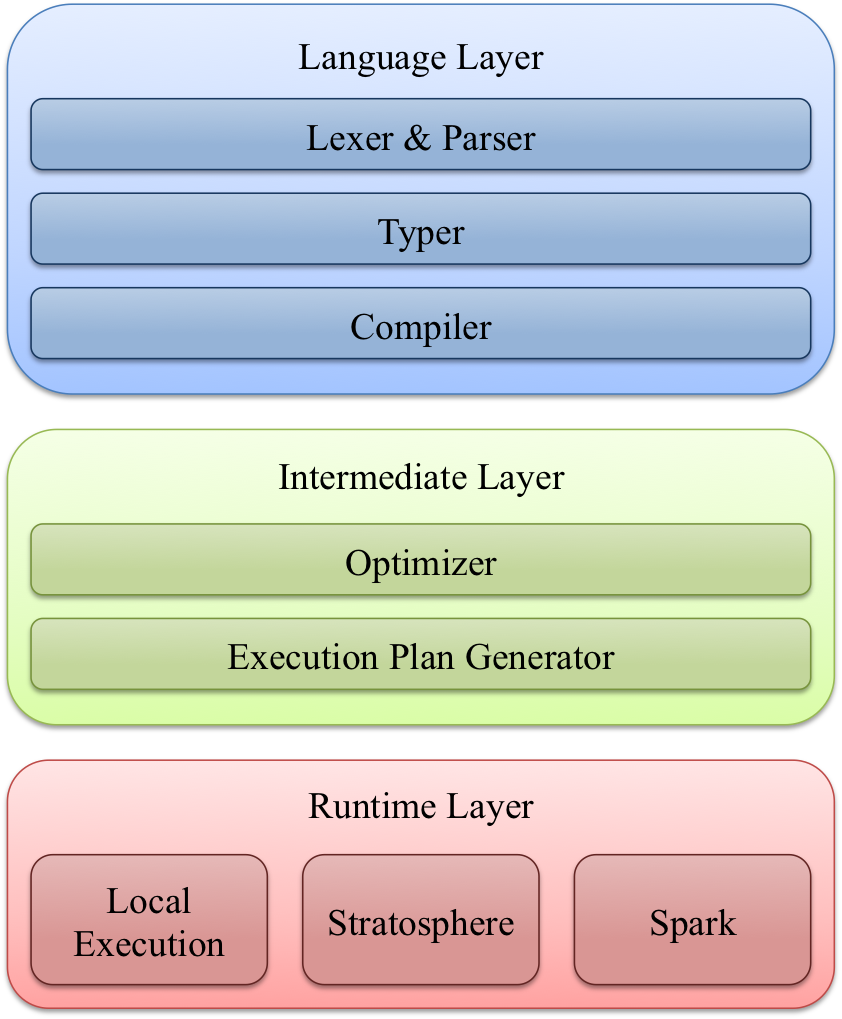
\includegraphics[height=0.175\paperheight]{images/systemArchitecture.png}
	\caption{The layered system architecture of Gilbert. The language layer is responsible for parsing, typing and compiling the given Matlab code. The intermediate layer facilitates high-level optimization strategies. The runtime layer is responsible for executing the specified program in parallel.}
	\label{fig:systemArchitecture}
\end{figure}

The first layer is the language layer.
It contains all functionality to parse the given Gilbert code and to compile it into the IR.
The second layer is the intermediate layer and it receives the IR of the Gilbert code.
The intermediate format is the ideal representation to apply language independent high-level transformations.
The Gilbert optimizer applies several algebraic optimizations prior to the generation of the execution plan.
The execution plan generator translates the optimized IR into a specific execution plan, depending on the selected execution engine.
Once the program has been translated into an execution engine's specific plan, it is executed on the respective back end.

\subsection{Language Layer}

The language layer contains all the logic for translating Gilbert source code into the intermediate representation, see \cref{cha:intermediaterepresentation} for more details.
Gilbert's supported language and its features is described in \cref{sec:gilbertLanguage}.

The resulting AST is attributed with type information by the typing system.
The typer makes use of the Hindley-Milner algorithm to automatically infer types, as it is described in~\cref{sec:hmInference}.
The type information enriched AST is then translated into a front end independent representation of linear algebra operations, namely the IR.
The format Gilbert uses to represent linear algebra operations in a generalized format is described in \cref{sec:intermediaterepresentation}.

\subsection{Intermediate Layer}

The intermediate layer contains the optimizer and the execution plan generator.
The optimizer applies the optimizations described in \cref{cha:optimizer} to IR of the Gilbert program.
Then the IR is translated into the execution engine's specific format.
The linear algebra operations are translated into a dataflow graph as explained in \cref{sec:operatorImplementation}.
The system supports Flink and Spark as parallel execution engines.